% Project structure
%!TEX root = ../Project.tex
\section{Project Structure \& Specification}
\label{sec:project_structure___specification}

This appendix contain all the technical information of a `project' and the data format used.

\begin{figure}[htbp]
	\centering
		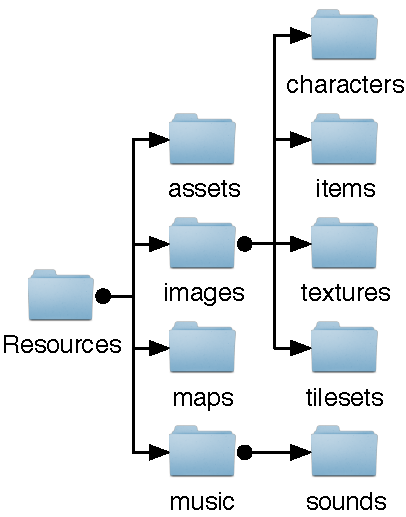
\includegraphics[height=3in]{figures/Files.pdf}
	\caption{Project Structure}
	\label{fig:figures_Files}
\end{figure}

A game's resources  are organised as shown above. One of the main restrictions, is that all external links have to be relative to \texttt{resources} directory. All \texttt{xml} files \textbf{must} conform in the schemas in the \texttt{schemas} directory. 


\subsection{Assets}
Assets are store in following format:
\begin{lst:resource}[caption=Assets format]
<name>
  <entry>
    <uuid>128bit</uuid> 
    <resource uuid="128 bit">
    </resource>
  </entry>
</name>
\end{lst:resource}

The \texttt{assets} directory \textbf{must} contain the following files conforming to schemas in \texttt{schemas/assets}.
\begin{lstlisting}[caption=Required Assets]
maps.xml
music.xml
ordering.xml
skills.xml
sounds.xml
textures.xml
tilesets.xml
units.xml
unitsImages.xml
weapons.xml
\end{lstlisting}

\subsection{images}
All images are stored as sprite sheets(see section \ref{ssub:sprite_sheets}).  There \emph{three} required files for each sprite sheet. 
\begin{lstlisting}
name.png
name.xml
name-animations.xml
\end{lstlisting}
The sprite sheet itself is stored as  a png(Portable Network Graphics) in \texttt{name.png}. \texttt{name.xml} contains the coordinates of each images in the sheet as well as the dimensions of the sheet. \texttt{name-animations.xml} contains the unique id of the sprite sheet and can optional specify animations. 

\subsection{Maps}
\label{sub:amaps}

Each map needs the following \emph{five} files:
\begin{description}
	\item[name.xml] which contains the tile data as well references to the other files. 
	\item[name-conditions.xml]  which include among other information, the  winning conditions. 
	\item[default-enemies.xml]  which contains the enemies data along with their positions on the map.
	\item[default-events.xml]   which optionally contains the dialog which is shon the start and end of battle
	\item[default-music.xml]    which contains the background music and sound effect.
\end{description}

Maps also need a \texttt{tilemaping} which maps the tile's type to their images.  A default \texttt{tilemaping} is created by the editor when a tileset is saved with the name \texttt{tileset-mapping.xml}.

\subsection{Music}
The engine supports only Ogg Vorbis which is ``a completely open, patent-free, professional audio encoding and streaming technology''\cite{ogg}.
Compared with other format such as MP3, Ogg Vorbis has no lieancely issues. 

\subsection{Sound Effects}
Sound effect can either be Ogg Vorbis, or wave(.wav) format. Sound effect should be less then 7 seconds, otherwise the sound effect may be truncated. 

\clearpage
\subsection{Editor}
For the editor the follow structure is used.

\begin{figure}[htbp]
	\centering
		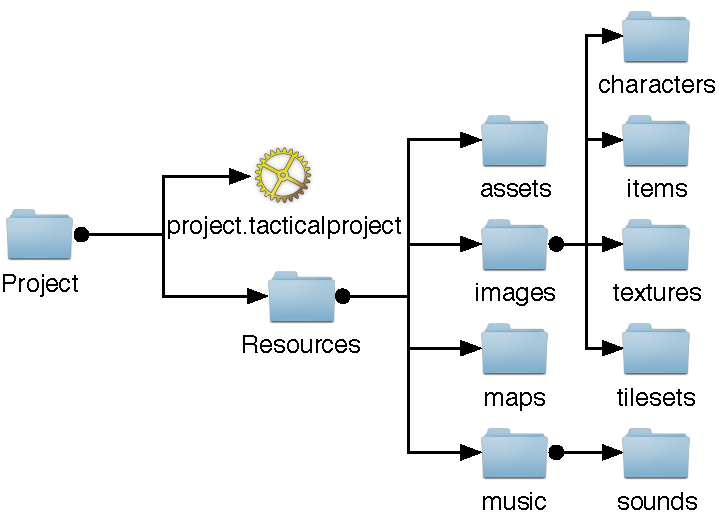
\includegraphics[height=3in]{figures/project.pdf}
	\caption{Editor Project Structure}
	\label{fig:figures_project}
\end{figure}

The main change is the addition of \texttt{project.tacticalproject} file which contains settings specific to the editor. It also has the added benefit of allows the user to click on the \texttt{project.tacticalproject} to open the editor if using the Mac version.

\subsubsection{Dialog Data Format}
\label{ssub:dialog_data_format}

The data format is actually YAML\cite{yaml}. This allows more formatting options as well the single format discussed previous. The advantage of using YAML is that there are parser aviable for java\cite{snake}. This saved development time since I did not have to built a parser. The main advantage of YAML is that is very characters that need to be escaped namely \textbf{:} if it appears at the start of the dialog's text or speaker's name. \textbf{\#} also has to be escaped since it the comment character in \texttt{YAML}. Since they character are fairly uncommon in dialog, it should not pose to much hassle to the user. In any case the use  the form \texttt{- Speaker: |-} then  write the text on an intended line which escapes all characters in the block.

\begin{lstlisting}[caption=A example show the features of the dialog's data format]
- Speaker:   Some text.
- none:      no speaker.
- New Enemy 2: |-
    "All the text in this block (until two newlines),
    are part of New Enemy 2's dialog". 
    No characters need to be escaped in this block e.g #  : \

- Other speaker: Even more text.
\end{lstlisting}
Specify the must satisfy the following:
\begin{itemize}
	\item  At lest one portion of text. A empty file is invaild
	\item  Each portion of text must have a speaker identified by their name or \texttt{none} for no speaker.
	\item  No other elements are allowed.
\end{itemize}

When the dialog is imported, if there a unit with  the specified name it is associated with the  portion of text otherwise the text is treated as having no speaker.
